% fig_predictions.tex -- forest panel removed, schematic only.
% Two parts: (a) the ratio prediction as one schematic (matched cells equal: dotted segment flat); (b) forest plot of
% the matched-cell AUROC (Q750|C750 above Q250|C250; 0.5 = ratio prediction) for W1(H0) and L_max(H0), 4 corpora x
% 5 models x 2 arms. Data: data/ratio_forest.dat from real_data.py <- reference_outputs/realtext_stats_summary.md Table S0 (columns
% 'W1 diag', 'longbar diag'; 95% document-bootstrap intervals). Vermillion = the ratio prediction only.
% \input from main.tex (no preamble here). axes moved 0.6 cm right so the key clears the corpus labels.
\providecommand{\didpath}{figs_didactic/}%
\definecolor{didV}{HTML}{D55E00}\definecolor{didB}{HTML}{0072B2}%
\input{\didpath data/ratio_forest_meta.tex}% corpora, ticks, labels, height (written by real_data.py)
\pgfplotsset{didforest/.style={scale only axis, width=4.4cm, height=\rfHeight, xmin=0, xmax=1, ymin=-0.9, ymax=\rfYmax,
  y dir=reverse, axis x line=bottom, axis y line=left, y axis line style={draw=none}, ytick style={draw=none},
  x axis line style={line width=0.4pt, black!70, -}, xtick style={line width=0.4pt, black!70}, major tick length=2pt,
  xtick={0,0.25,0.5,0.75,1}, xticklabels={$0$,,$0.5$,,$1$}, clip=false,
  tick label style={font=\footnotesize}, label style={font=\footnotesize},
  ytick/.expand once=\rfYticks},
  didfp/.style={only marks, mark=*, mark size=1.45pt, didB, error bars/.cd, x dir=both, x explicit,
    error bar style={line width=0.45pt, didB}, error mark=none},
  didfl/.style={only marks, mark=*, mark size=1.45pt, mark options={fill=white, draw=didB, line width=0.6pt},
    didB, error bars/.cd, x dir=both, x explicit, error bar style={line width=0.45pt, didB!70}, error mark=none}}%
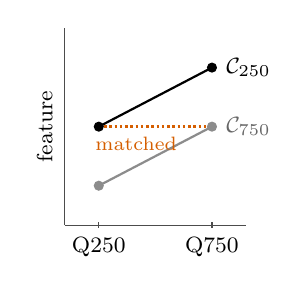
\begin{tikzpicture}[font=\footnotesize]
  % ---------------- (a) the ratio prediction, schematic ----------------
  \begin{axis}[scale only axis, width=2.3cm, height=2.5cm, at={(0cm,4.2cm)}, anchor=south west, xmin=-0.3, xmax=1.3,
      ymin=0, ymax=1, axis lines=left, axis line style={line width=0.4pt, black!70, -},
      tick style={line width=0.4pt, black!70}, major tick length=2pt, xtick={0,1}, xticklabels={Q250, Q750},
      ytick=\empty, ylabel={feature}, clip=false, label style={font=\footnotesize}, tick label style={font=\footnotesize}]
    \addplot[line width=0.8pt, black, mark=*, mark size=1.4pt] coordinates {(0,0.5) (1,0.8)};
    \addplot[line width=0.8pt, black!45, mark=*, mark size=1.4pt] coordinates {(0,0.2) (1,0.5)};
    \addplot[line width=0.9pt, didV, densely dotted] coordinates {(0,0.5) (1,0.5)};
    \node[anchor=west] at (axis cs:1.04,0.8) {$\mathcal{C}_{250}$};
    \node[anchor=west, text=black!60] at (axis cs:1.04,0.5) {$\mathcal{C}_{750}$};
    \node[anchor=north, inner sep=1pt, text=didV, font=\scriptsize] at (axis cs:0.33,0.465) {matched};  % moved into the gap above the dotted line
  \end{axis}
\end{tikzpicture}%
